\documentclass[11pt,a4paper]{report}
\usepackage[textwidth=37em,vmargin=30mm]{geometry}
\usepackage{calc,xunicode,amsmath,amssymb,paralist,enumitem,tabu,booktabs,datetime2,xeCJK,xeCJKfntef,listings}
\usepackage{tocloft,fancyhdr,tcolorbox,xcolor,graphicx,eso-pic,xltxtra,xelatexemoji}

\newcommand{\envyear}[0]{2024}
\newcommand{\envdatestr}[0]{2024-10-22}
\newcommand{\envfinaldir}[0]{webdb/2024/20241022/final}

\usepackage[hidelinks]{hyperref}
\hypersetup{
    colorlinks=false,
    pdfpagemode=FullScreen,
    pdftitle={Web Digest - \envdatestr}
}

\setlength{\cftbeforechapskip}{10pt}
\renewcommand{\cftchapfont}{\rmfamily\bfseries\large\raggedright}
\setlength{\cftbeforesecskip}{2pt}
\renewcommand{\cftsecfont}{\sffamily\small\raggedright}

\setdefaultleftmargin{2em}{2em}{1em}{1em}{1em}{1em}

\usepackage{xeCJK,xeCJKfntef}
\xeCJKsetup{PunctStyle=plain,RubberPunctSkip=false,CJKglue=\strut\hskip 0pt plus 0.1em minus 0.05em,CJKecglue=\strut\hskip 0.22em plus 0.2em}
\XeTeXlinebreaklocale "zh"
\XeTeXlinebreakskip = 0pt


\setmainfont{Brygada 1918}
\setromanfont{Brygada 1918}
\setsansfont{IBM Plex Sans}
\setmonofont{JetBrains Mono NL}
\setCJKmainfont{Noto Serif CJK SC}
\setCJKromanfont{Noto Serif CJK SC}
\setCJKsansfont{Noto Sans CJK SC}
\setCJKmonofont{Noto Sans CJK SC}

\setlength{\parindent}{0pt}
\setlength{\parskip}{8pt}
\linespread{1.15}

\lstset{
	basicstyle=\ttfamily\footnotesize,
	numbersep=5pt,
	backgroundcolor=\color{black!5},
	showspaces=false,
	showstringspaces=false,
	showtabs=false,
	tabsize=2,
	captionpos=b,
	breaklines=true,
	breakatwhitespace=true,
	breakautoindent=true,
	linewidth=\textwidth
}






\newcommand{\coverpic}[2]{
    % argv: itemurl, authorname
    Cover photo by #2~~(\href{#1}{#1})
}
\newcommand{\makeheader}[0]{
    \begin{titlepage}
        % \newgeometry{hmargin=15mm,tmargin=21mm,bmargin=12mm}
        \begin{center}
            
            \rmfamily\scshape
            \fontspec{BaskervilleF}
            \fontspec{Old Standard}
            \fontsize{59pt}{70pt}\selectfont
            WEB\hfill DIGEST
            
            \vfill
            % \vskip 30pt
            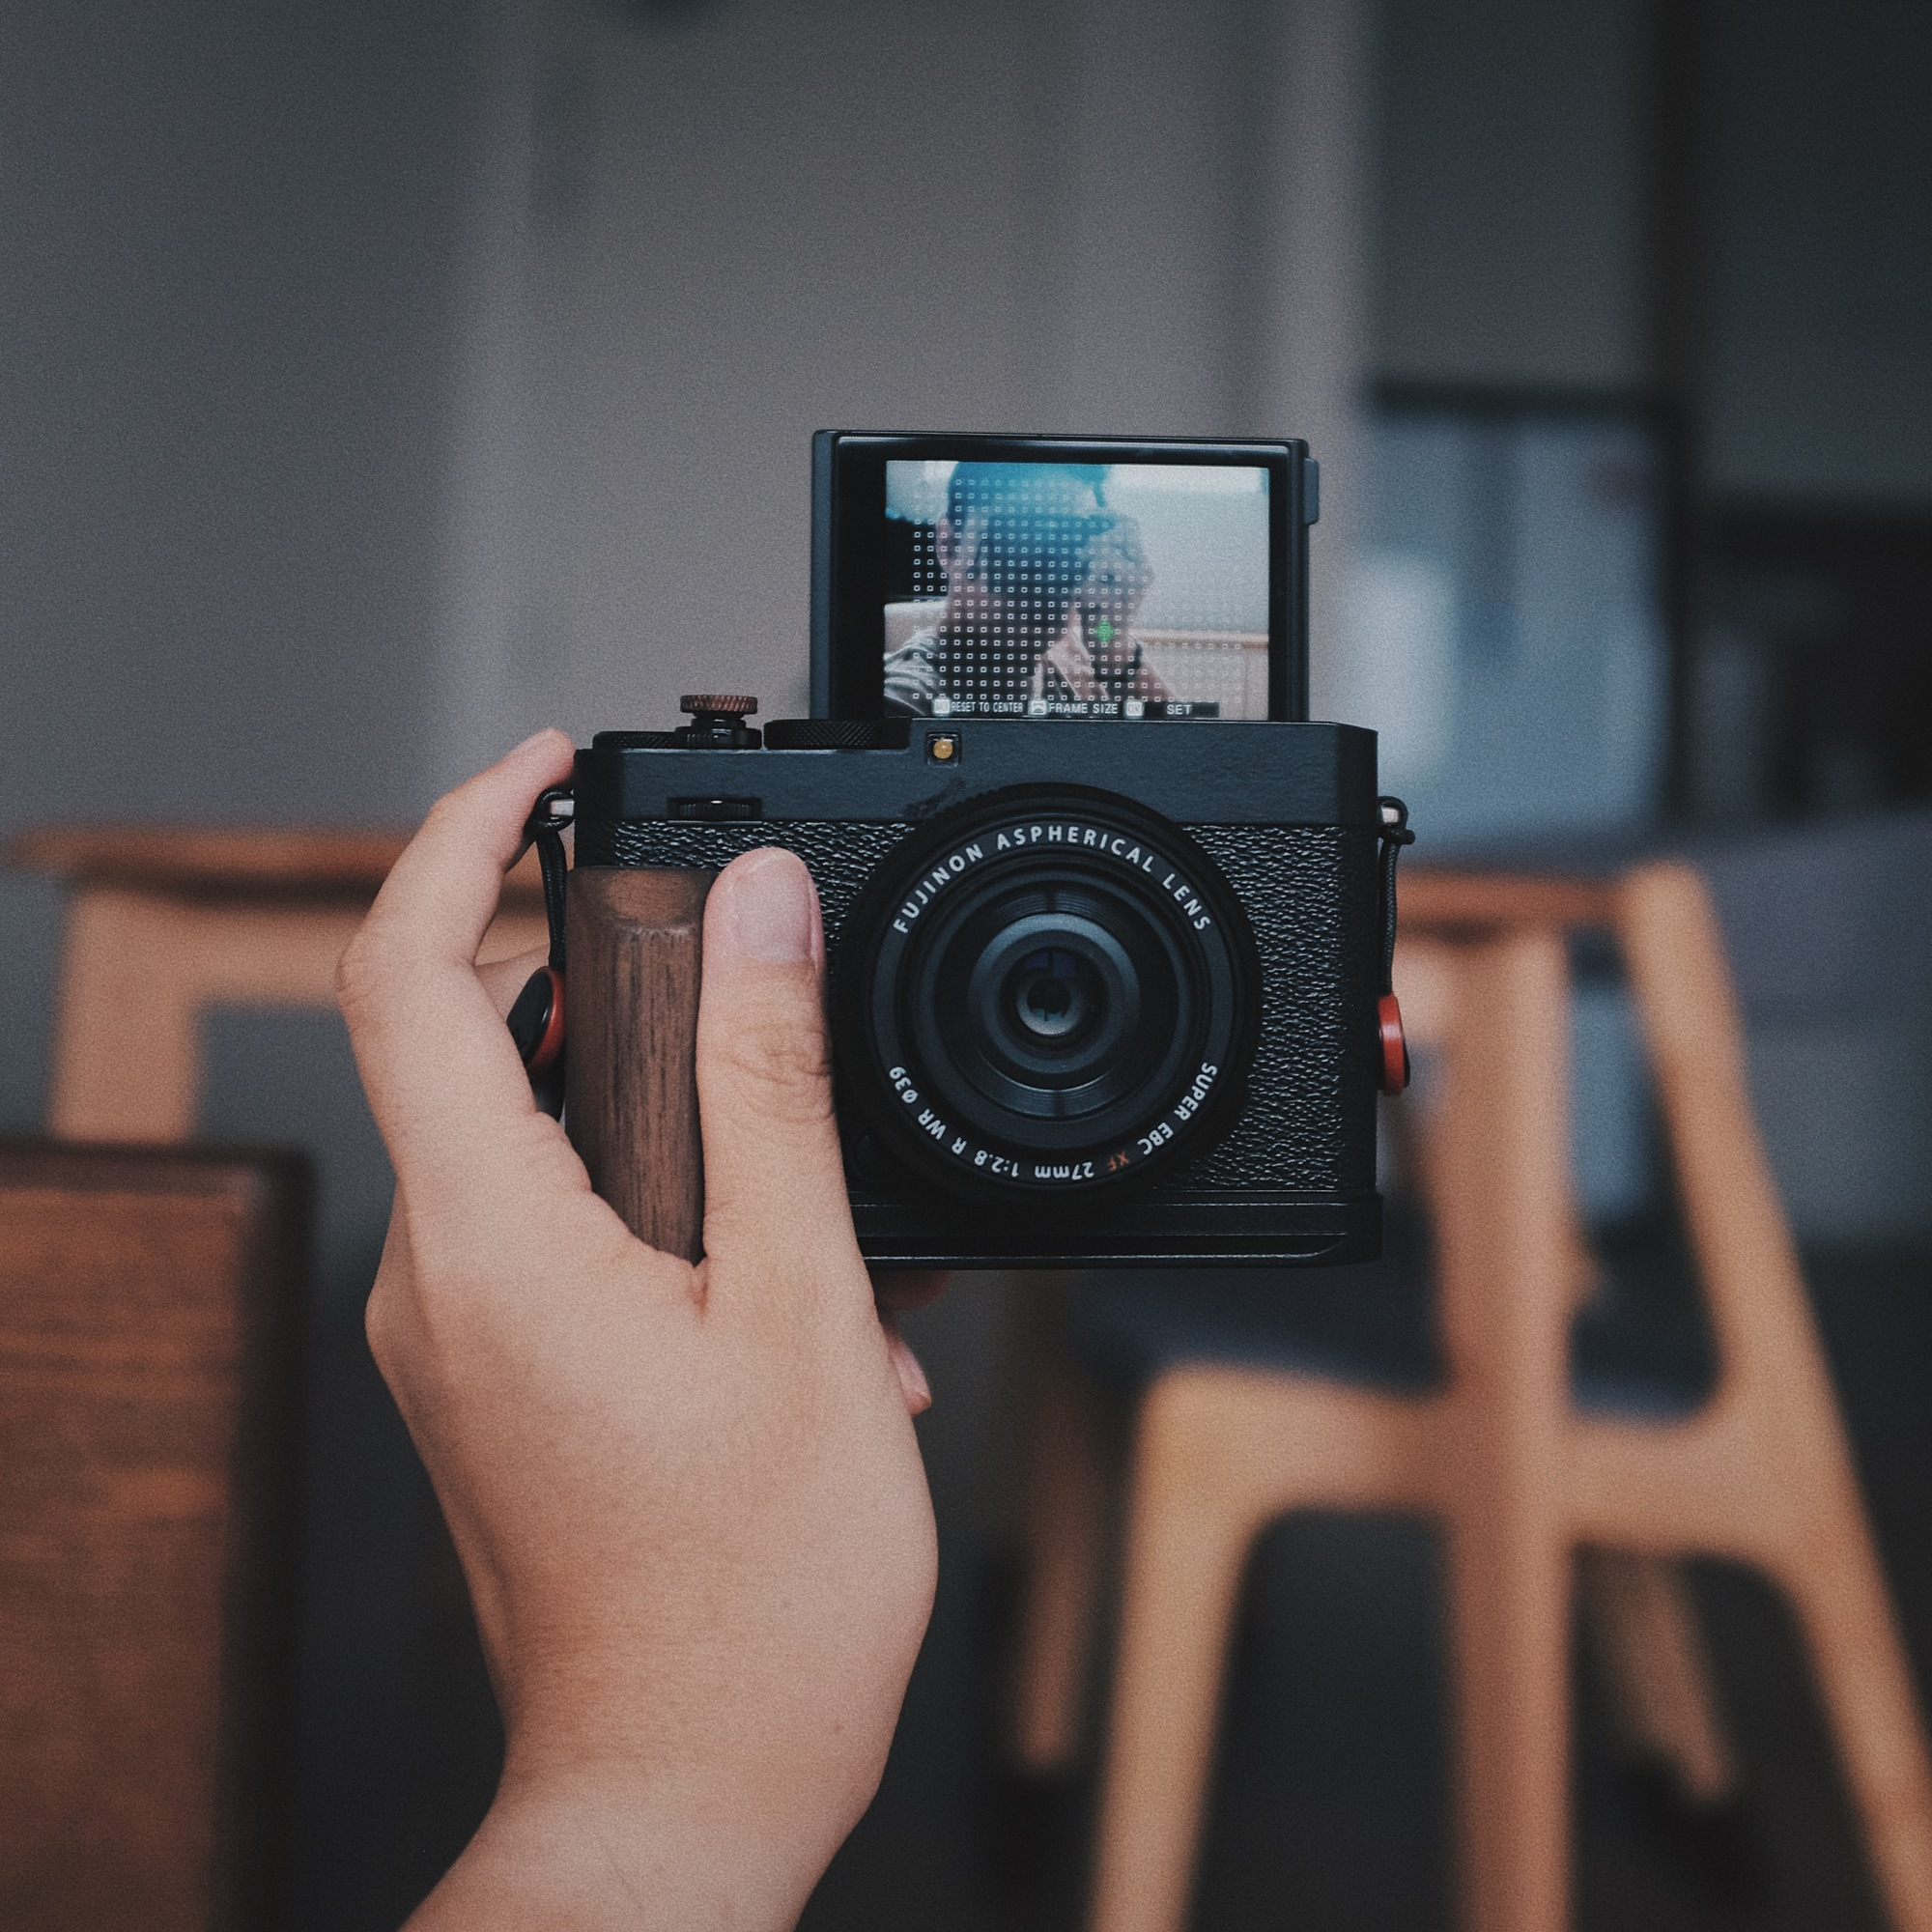
\includegraphics[width=\linewidth]{\envfinaldir/coverpic-prod.jpg}\par
            % \vskip 30pt
            \vfill

            \normalsize\rmfamily\scshape
            \copyright{} The Web Digest Project \hfill\large \envdatestr
        \end{center}
    \end{titlepage}
    % \restoregeometry
}
\newcommand{\simplehref}[1]{%
    \textcolor{blue!80!green}{\href{#1}{#1}}%
}
\renewcommand{\contentsname}{\center\Huge\sffamily\bfseries Contents\par\vskip 20pt}
\newcounter{ipartcounter}
\setcounter{ipartcounter}{0}
\newcommand{\ipart}[1]{
    % \vskip 20pt
    \clearpage
    \stepcounter{ipartcounter}
    \phantomsection
    \addcontentsline{toc}{chapter}{#1}
    % \begin{center}
    %     \Huge
    %     \sffamily\bfseries
    %     #1
    % \end{center}
    % \vskip 20pt plus 7pt
}
\newcounter{ichaptercounter}
\setcounter{ichaptercounter}{0}
\newcommand{\ichapter}[1]{
    % \vskip 20pt
    \clearpage
    \stepcounter{ichaptercounter}
    \phantomsection
    \addcontentsline{toc}{section}{\numberline{\arabic{ichaptercounter}}#1}
    \begin{center}
        \Huge
        \sffamily\bfseries
        #1
    \end{center}
    \vskip 20pt plus 7pt
}
\newcommand{\entrytitlefont}[1]{\subsection*{\raggedright\Large\sffamily\bfseries#1}}
\newcommand{\entryitemGeneric}[2]{
    % argv: title, url
    \parbox{\linewidth}{
        \entrytitlefont{#1}\par\vskip 5pt
        \footnotesize\ttfamily\mdseries
        \simplehref{#2}
    }\vskip 11pt plus 11pt minus 1pt
}
\newcommand{\entryitemGithub}[3]{
    % argv: title, url, desc
    \parbox{\linewidth}{
        \entrytitlefont{#1}\par\vskip 5pt
        \footnotesize\ttfamily\mdseries
        \simplehref{#2}\par\vskip 5pt
        \small\rmfamily\mdseries#3
    }\vskip 11pt plus 11pt minus 1pt
}
\newcommand{\entryitemAp}[3]{
    % argv: title, url, desc
    \parbox{\linewidth}{
        \entrytitlefont{#1}\par\vskip 5pt
        \footnotesize\ttfamily\mdseries
        \simplehref{#2}\par\vskip 5pt
        \small\rmfamily\mdseries#3
    }\vskip 11pt plus 11pt minus 1pt
}
\newcommand{\entryitemHackernews}[3]{
    % argv: title, hnurl, rawurl
    % \parbox{\linewidth}{
    %     \entrytitlefont{#1}\par\vskip 5pt
    %     \footnotesize\ttfamily\mdseries
    %     \simplehref{#3}\par
    %     \textcolor{black!50}{\href{#2}{#2}}
    % }\vskip 11pt plus 11pt minus 1pt
    \begin{minipage}{\linewidth}
            \entrytitlefont{#1}\par\vskip 5pt
            \footnotesize\ttfamily\mdseries
            \simplehref{#3}\par
            \textcolor{black!50}{\href{#2}{#2}}
    \end{minipage}\par\vskip 11pt plus 11pt minus 1pt
}







\begin{document}

\makeheader

\tableofcontents\clearpage




\ipart{Developers}
\ichapter{Hacker News}
\entryitemTwoLinks{T-Mobile, AT\&T oppose unlocking rule, claim locked phones are good for users}{https://news.ycombinator.com/item?id=41908231}{https://arstechnica.com/tech-policy/2024/10/t-mobile-att-oppose-unlocking-rule-claim-locked-phones-are-good-for-users/}

\entryitemTwoLinks{Overengineering a way to know if people are in my university's CS lab}{https://news.ycombinator.com/item?id=41907360}{https://www.amoses.dev/blog/upl-people-counter/}

\entryitemTwoLinks{Microsoft is introducing hidden APIs to VS Code only enabled for Copilot?}{https://news.ycombinator.com/item?id=41907350}{https://old.reddit.com/r/ChatGPTCoding/comments/1g8xrub/microsoft\_is\_introducing\_hidden\_apis\_to\_vs\_code/}

\entryitemTwoLinks{Please do not write below the line}{https://news.ycombinator.com/item?id=41907071}{http://www.bbctvlicence.com/Please\%20do\%20not\%20write\%20below\%20the\%20line.htm}

\entryitemTwoLinks{U.S. border surveillance towers have always been broken}{https://news.ycombinator.com/item?id=41906283}{https://www.eff.org/deeplinks/2024/10/us-border-surveillance-towers-have-always-been-broken}

\entryitemTwoLinks{An amateur historian has discovered a long-lost short story by Bram Stoker}{https://news.ycombinator.com/item?id=41905664}{https://www.bbc.com/news/articles/c4g9119l64qo}

\entryitemTwoLinks{Can SpaceX land a rocket with 1/2 cm accuracy?}{https://news.ycombinator.com/item?id=41905215}{https://theshamblog.com/can-spacex-land-a-rocket-with-1-2-cm-accuracy/}

\entryitemTwoLinks{Intelsat 33e breaks up in geostationary orbit}{https://news.ycombinator.com/item?id=41904346}{https://spacenews.com/intelsat-33e-loses-power-in-geostationary-orbit/}

\entryitemTwoLinks{Show HN: Epublifier – scrape pages (books, manuals) for offline reading}{https://news.ycombinator.com/item?id=41903864}{https://github.com/maoserr/epublifier}

\entryitemTwoLinks{Egypt declared malaria-free after 100-year effort}{https://news.ycombinator.com/item?id=41903616}{https://www.bbc.com/news/articles/cm2yl8pjgn2o}

\entryitemTwoLinks{IOCCC Flight Simulator (2010)}{https://news.ycombinator.com/item?id=41903399}{https://blog.aerojockey.com/iocccsim/}

\entryitemTwoLinks{Show HN: Erin – Open-source and self-hosted TikTok feed for your own videos}{https://news.ycombinator.com/item?id=41902407}{https://github.com/will-moss/erin}

\entryitemTwoLinks{AWS and Azure Are at Least 4x–10x More Expensive Than Hetzner}{https://news.ycombinator.com/item?id=41902103}{https://learn.umh.app/course/aws-and-azure-are-at-least-4x-10x-more-expensive-than-hetzner/}

\entryitemTwoLinks{Google Drive Blackout in Italy After Another Major Anti-Piracy Blunder}{https://news.ycombinator.com/item?id=41901168}{https://torrentfreak.com/google-drive-blackout-in-italy-after-another-major-anti-piracy-blunder-241020/}

\entryitemTwoLinks{Software engineer titles have almost lost all their meaning}{https://news.ycombinator.com/item?id=41900456}{https://www.trevorlasn.com/blog/software-engineer-titles-have-almost-lost-all-their-meaning}

\entryitemTwoLinks{Scientists working to decode birdsong}{https://news.ycombinator.com/item?id=41900404}{https://www.newyorker.com/magazine/2024/10/21/how-scientists-started-to-decode-birdsong}

\entryitemTwoLinks{ByteDance sacks intern for sabotaging AI project}{https://news.ycombinator.com/item?id=41900402}{https://www.bbc.com/news/articles/c7v62gg49zro}

\entryitemTwoLinks{A step toward fully 3D-printed active electronics}{https://news.ycombinator.com/item?id=41899873}{https://news.mit.edu/2024/mit-team-takes-major-step-toward-fully-3d-printed-active-electronics-1015}

\entryitemTwoLinks{Learn Rust the Dangerous Way}{https://news.ycombinator.com/item?id=41899599}{https://cliffle.com/p/dangerust/}

\entryitemTwoLinks{Today is Ubuntu's 20th Anniversary}{https://news.ycombinator.com/item?id=41898736}{https://lists.ubuntu.com/archives/ubuntu-announce/2004-October/000003.html}\ichapter{Phoronix}
\entryitemGeneric{\hskip 0pt{}SiFive HiFive Premier P550 RISC-V Development Board Update}{https://www.phoronix.com/news/SiFive-Premier-P550-Update}

\entryitemGeneric{\hskip 0pt{}Intel Core Ultra 7 256V Lunar Lake With ASUS Zenbook Performing Better After New Linux Patch}{https://www.phoronix.com/review/intel-lunar-lake-aipt-xe2}

\entryitemGeneric{\hskip 0pt{}AMD Posts Linux Patches For EPYC To Further Enhance Performance-Per-Watt By Default}{https://www.phoronix.com/news/AMD-P-State-EPYC-Linux-Patches}

\entryitemGeneric{\hskip 0pt{}Intel IWD 3.0 Wireless Daemon Released For Linux Systems}{https://www.phoronix.com/news/Intel-IWD-3.0}

\entryitemGeneric{\hskip 0pt{}Linus Torvalds Growing Frustrated By Buggy Hardware \& Theoretical CPU Attacks}{https://www.phoronix.com/news/Torvalds-Frustrated-Buggy-HW}

\entryitemGeneric{\hskip 0pt{}Hangover 9.20 Restores Support For Running Win64 Applications On ARM64 Wine}{https://www.phoronix.com/news/Hangover-9.20-Win64-On-ARM64}

\entryitemGeneric{\hskip 0pt{}Unvanquished 0.55 Released With Big Performance Optimizations For Its Engine}{https://www.phoronix.com/news/Unvanquished-0.55-Released}

\entryitemGeneric{\hskip 0pt{}Meson 1.6 Build System Adds Support For Flang \& OpenXL Compilers}{https://www.phoronix.com/news/Meson-1.6-Released}

\entryitemGeneric{\hskip 0pt{}Linux 6.12-rc4 Released With MSI Claw A1M Controller Support, Intel \& AMD Fixes}{https://www.phoronix.com/news/Linux-6.12-rc4-Released}


\ipart{Developers~~~~(zh-Hans)}
\ichapter{Solidot}
\entryitemGeneric{\hskip 0pt{}Linux 6.13 预计将移除 ReiserFS 文件系统}{https://www.solidot.org/story?sid=79548}

\entryitemGeneric{\hskip 0pt{}GNU Boot 再次发现包含非自由代码}{https://www.solidot.org/story?sid=79547}

\entryitemGeneric{\hskip 0pt{}字节跳动以恶意干扰 AI 模型训练为由解雇了一名实习生}{https://www.solidot.org/story?sid=79546}

\entryitemGeneric{\hskip 0pt{}更多证据表明长新冠是一种脑损伤}{https://www.solidot.org/story?sid=79545}

\entryitemGeneric{\hskip 0pt{}微软用蜜罐大规模欺骗钓鱼者}{https://www.solidot.org/story?sid=79544}

\entryitemGeneric{\hskip 0pt{}在致命车祸后美国调查特斯拉的 Full Self-Driving 软件}{https://www.solidot.org/story?sid=79543}

\entryitemGeneric{\hskip 0pt{}Ubuntu 发布二十周年}{https://www.solidot.org/story?sid=79542}

\entryitemGeneric{\hskip 0pt{}芯片设计师回顾了英特尔和 AMD 之间围绕 x86-64 的竞争}{https://www.solidot.org/story?sid=79541}

\entryitemGeneric{\hskip 0pt{}古巴大范围断电已持续三天}{https://www.solidot.org/story?sid=79540}

\entryitemGeneric{\hskip 0pt{}82 岁老妇仍然骑 13 岁时父母送的自行车}{https://www.solidot.org/story?sid=79539}

\entryitemGeneric{\hskip 0pt{}德国主权科技基金过去两年向开源项目资助了逾  2300 万欧元}{https://www.solidot.org/story?sid=79538}

\entryitemGeneric{\hskip 0pt{}OpenAI 相对于其它 AI 公司的优势基本消失}{https://www.solidot.org/story?sid=79537}

\entryitemGeneric{\hskip 0pt{}古巴电网故障导致千万人断电}{https://www.solidot.org/story?sid=79536}

\entryitemGeneric{\hskip 0pt{}美国越来越多的父母拒绝给孩子接种疫苗}{https://www.solidot.org/story?sid=79535}\ichapter{V2EX}
\entryitemGeneric{\hskip 0pt{}[Linux] Traefik 代理 smtps 和 imaps 等邮箱协议}{https://www.v2ex.com/t/1082379}

\entryitemGeneric{\hskip 0pt{}[程序员] VScode 有个插件能智能展示函数调用堆栈的, 请问是哪个插件}{https://www.v2ex.com/t/1082378}

\entryitemGeneric{\hskip 0pt{}[Samsung] 三星不支持 Call over Cellular Data 吗?}{https://www.v2ex.com/t/1082376}

\entryitemGeneric{\hskip 0pt{}[程序员] 自从主力切换到 MacBook 后到哪都带着笔记本,接个外显生产力拉满; Mac mini 还有啥购买必要呢?}{https://www.v2ex.com/t/1082375}

\entryitemGeneric{\hskip 0pt{}[问与答] 我很好奇,超过 30+的人,目前状况如何。}{https://www.v2ex.com/t/1082374}

\entryitemGeneric{\hskip 0pt{}[职场话题] 国内后端就业现在什么行情? Java 还是最佳技能吗?}{https://www.v2ex.com/t/1082372}

\entryitemGeneric{\hskip 0pt{}[求职] [求职远程]全栈程序员求职远程办公工作}{https://www.v2ex.com/t/1082371}

\entryitemGeneric{\hskip 0pt{}[问与答] 有没有老哥帮忙看下微信小程序``极简云待办 TODO''可能是用什么 UI 框架写的?}{https://www.v2ex.com/t/1082370}

\entryitemGeneric{\hskip 0pt{}[macOS] mac 全屏播放视频,右上角有个小蓝点}{https://www.v2ex.com/t/1082369}

\entryitemGeneric{\hskip 0pt{}[问与答] 这种比较激进的风扇策略行不行?}{https://www.v2ex.com/t/1082368}

\entryitemGeneric{\hskip 0pt{}[Go 编程语言] 有没有用 wails 做桌面客户端播放视频全屏只能窗口全屏问题的?}{https://www.v2ex.com/t/1082367}

\entryitemGeneric{\hskip 0pt{}[程序员] 请问海钓的论坛有吗?}{https://www.v2ex.com/t/1082366}

\entryitemGeneric{\hskip 0pt{}[杭州] 杭州 E 类人才通过什么材料怎么申请快}{https://www.v2ex.com/t/1082365}

\entryitemGeneric{\hskip 0pt{}[程序员] [出海记录]开发新手的第八个站点上线}{https://www.v2ex.com/t/1082364}

\entryitemGeneric{\hskip 0pt{}[Firefox] 2024 年,谋智火狐还``活着''吗?}{https://www.v2ex.com/t/1082363}

\entryitemGeneric{\hskip 0pt{}[Windows] 急! Win Server22 帐户自动锁定是什么情况?}{https://www.v2ex.com/t/1082362}

\entryitemGeneric{\hskip 0pt{}[宽带症候群] 家庭全屋 AP+NAS+路由应该怎么组网,求帮助}{https://www.v2ex.com/t/1082361}

\entryitemGeneric{\hskip 0pt{}[程序员] 微服务到底在哪个方面让开发、维护简单了?怎么看都是变复杂了,原本配置一次数据库就能跑,现在要配置八九个容器和数据库,更新一次要配置好几个服务}{https://www.v2ex.com/t/1082359}

\entryitemGeneric{\hskip 0pt{}[程序员] 用 cursor 开发了一个语义化搜索书签的 chrome 插件,已开源}{https://www.v2ex.com/t/1082357}

\entryitemGeneric{\hskip 0pt{}[分享创造] [分享] 我做了一个我的世界(Minecraft)风格的 2048 游戏,欢迎来玩!}{https://www.v2ex.com/t/1082356}

\entryitemGeneric{\hskip 0pt{}[互联网] 小红书开始无法访问直链了}{https://www.v2ex.com/t/1082355}

\entryitemGeneric{\hskip 0pt{}[问与答] [来瞧瞧] 网址接入微信登录功能,发现 PC 端微信监听的一个接口很奇怪}{https://www.v2ex.com/t/1082354}

\entryitemGeneric{\hskip 0pt{}[淘宝] 淘宝下单失败}{https://www.v2ex.com/t/1082353}

\entryitemGeneric{\hskip 0pt{}[分享创造] 小程序版进销存系统,俗称门店记账系统,有搞头吗?}{https://www.v2ex.com/t/1082352}

\entryitemGeneric{\hskip 0pt{}[Android] 个人向的 vivo X200 Pro 优缺点总结}{https://www.v2ex.com/t/1082351}

\entryitemGeneric{\hskip 0pt{}[NAS] 收 unraid plus 或者 pro 版}{https://www.v2ex.com/t/1082349}

\entryitemGeneric{\hskip 0pt{}[Apple] 日思夜想盼 Mac mini...}{https://www.v2ex.com/t/1082348}

\entryitemGeneric{\hskip 0pt{}[问与答] 为什么很多 ui 的背景设计不使用纯白? 而是使用 fafafa ?}{https://www.v2ex.com/t/1082347}

\entryitemGeneric{\hskip 0pt{}[问与答] 吐槽,遇到个奇葩的开发模式~}{https://www.v2ex.com/t/1082345}

\entryitemGeneric{\hskip 0pt{}[分享创造] 做完了掌机 Miyoo 主题相关的所有游戏机图标,相当满足。}{https://www.v2ex.com/t/1082343}

\entryitemGeneric{\hskip 0pt{}[程序员] cursor 还是很给力的,终于不用担心不会写前端代码了}{https://www.v2ex.com/t/1082342}

\entryitemGeneric{\hskip 0pt{}[程序员] 我想把 GitHub 上看到的一个好用的、MIT 授权的、只有 CLI 的软件包装成一个完整的商业软件订阅制销售,以下做法违反 MIT 协议吗?}{https://www.v2ex.com/t/1082340}

\entryitemGeneric{\hskip 0pt{}[酷工作] [上海] 互联网金融公司 高级、资深 Java 工程师招聘,薪资 30~50k*15}{https://www.v2ex.com/t/1082339}

\entryitemGeneric{\hskip 0pt{}[Android] 小米对 Bootloader (BL) 跨区解锁权限施加了新限制}{https://www.v2ex.com/t/1082338}

\entryitemGeneric{\hskip 0pt{}[OpenWrt] immortalWrt 网卡频繁掉线上线,快要崩溃了,游戏根本玩不了一直掉线}{https://www.v2ex.com/t/1082337}

\entryitemGeneric{\hskip 0pt{}[优惠信息] 手快有,交行 3 元立减金!}{https://www.v2ex.com/t/1082336}

\entryitemGeneric{\hskip 0pt{}[宽带症候群] 重庆 网间互联带宽 900Gbps,省际直联带宽 51Tbps, 50 分之一都不到}{https://www.v2ex.com/t/1082335}

\entryitemGeneric{\hskip 0pt{}[分享创造] 花了两天时间做了一个标准规范批量查新的小工具}{https://www.v2ex.com/t/1082334}

\entryitemGeneric{\hskip 0pt{}[问与答] 可以推荐电脑适合长时间使用的配色吗}{https://www.v2ex.com/t/1082333}

\entryitemGeneric{\hskip 0pt{}[NAS] 21 元 diy 了一个钢结构的 NAS 机箱,旧笔记本电脑发挥余热!}{https://www.v2ex.com/t/1082332}

\entryitemGeneric{\hskip 0pt{}[职场话题] 什么样的工作是好工作}{https://www.v2ex.com/t/1082331}

\entryitemGeneric{\hskip 0pt{}[优惠信息] 今天天猫 MacBook Air 的价格比京东低 560}{https://www.v2ex.com/t/1082330}

\entryitemGeneric{\hskip 0pt{}[推广] [网站加速] Sheas Cealer 新进展 [开发近况分享]}{https://www.v2ex.com/t/1082329}

\entryitemGeneric{\hskip 0pt{}[Apple] 最终还是入了 iPad mini 2024 eSIM 版本,天猫店 92 折}{https://www.v2ex.com/t/1082328}

\entryitemGeneric{\hskip 0pt{}[分享创造] AI Hug Video Generator - https://aihugvideogenerator.com/}{https://www.v2ex.com/t/1082326}

\entryitemGeneric{\hskip 0pt{}[生活] 交通事故判责讨论,大家来瞅瞅。}{https://www.v2ex.com/t/1082324}

\entryitemGeneric{\hskip 0pt{}[宽带症候群] 北联通,南电信,名不虚传}{https://www.v2ex.com/t/1082323}

\entryitemGeneric{\hskip 0pt{}[ WATCH] Apple Watch 寄了还有办法抢救吗?}{https://www.v2ex.com/t/1082322}

\entryitemGeneric{\hskip 0pt{}[职场话题] 上周五面试到一家需要出差东南亚的公司,感觉是一个诈骗公司。问问大家有没有过相似的经历}{https://www.v2ex.com/t/1082320}

\entryitemGeneric{\hskip 0pt{}[分享发现] 为自己的博客增加 RSS 功能并在 follow 中 claim 自己的 feed}{https://www.v2ex.com/t/1082319}


\ipart{Generic News}
\ichapter{AP News}
\entryitemWithDescription{\hskip 0pt{}Duke's Cooper Flagg makes preseason AP All-America team as ACC, Big 12, SEC each place 2 players}{https://apnews.com/article/2b6f3922ae1bee8c6f8c8bb71449e2b1}{}

\entryitemWithDescription{\hskip 0pt{}Spielberg, Spike Lee and Queen Latifah among standouts in US arts and humanities honored by Biden}{https://apnews.com/article/59f514ce2282517bb1a23e125fbf9760}{}

\entryitemWithDescription{\hskip 0pt{}New Zealand airport imposes cuddle cap with 3-minute limit on goodbye hugs to avoid traffic jams}{https://apnews.com/article/d6176082ffb6ab66e8d2f05dd590b8aa}{}

\entryitemWithDescription{\hskip 0pt{}McDonald's agreed to Trump event but says it isn't endorsing a presidential candidate}{https://apnews.com/article/56a5773528e212df058f85ec0f264578}{}

\entryitemWithDescription{\hskip 0pt{}Facing 7 more lawsuits, Sean `Diddy' Combs protests a `fresh wave of publicity'}{https://apnews.com/article/0c25d256ee9351a64c30a8398c5a46d4}{}

\entryitemWithDescription{\hskip 0pt{}Writer Olivia Nuzzi, New York magazine part ways after relationship with political source revealed}{https://apnews.com/article/0eebc8e7a039b3170cfd037a4e0c416e}{}

\entryitemWithDescription{\hskip 0pt{}Susan Smith is up for parole 30 years after drowning her kids in a South Carolina lake}{https://apnews.com/article/ae37185c6d9d056104c839b03bd1cac0}{}

\entryitemWithDescription{\hskip 0pt{}New York Liberty win their first WNBA title and celebrate the end of a long odyssey}{https://apnews.com/article/64d2a724bc33bbec219dee826b5376ca}{}

\entryitemWithDescription{\hskip 0pt{}Directioners mourning singer Liam Payne leave tributes in London and other cities}{https://apnews.com/article/c14bec35ea2b14c27bf29368cfeed4b8}{}

\entryitemWithDescription{\hskip 0pt{}`Smile 2' grinning to No. 1 at box office while `Anora' glitters in limited release}{https://apnews.com/article/5ea3e6106c9714fb24ca6fe10765332c}{}

\entryitemWithDescription{\hskip 0pt{}One of the last Navajo Code Talkers from World War II dies at 107}{https://apnews.com/article/5f527f43eebaede11eb86f7bdad27a39}{}

\entryitemWithDescription{\hskip 0pt{}Dogs dressed to the nines for annual New York City Halloween event}{https://apnews.com/article/c703f6365b244d82e9c1ba6c0ceb56a1}{}

\entryitemWithDescription{\hskip 0pt{}Yehuda Bauer, prominent Israeli Holocaust scholar, dies at 98}{https://apnews.com/article/febc76ad8836b85019781f55599526ec}{}\ichapter{Reuters}
\entryitemWithDescription{\hskip 0pt{}Palestinians met requirements for Israel to extend banking waiver, source says}{https://www.reuters.com/world/middle-east/palestinians-met-requirements-israel-extend-banking-waiver-source-says-2024-10-21/}{Israel\textquotesingle s requirements for the indemnification needed to allow Israeli banks to continue conducting transactions with Palestinian banks have been met by the Palestinian authorities, according to a source familiar with the...}

\entryitemWithDescription{\hskip 0pt{}Russian attacks kill three in Zaporizhzhia, three in Donetsk region, officials say}{https://www.reuters.com/world/europe/russian-attacks-kill-three-zaporizhzhia-three-donetsk-region-officials-say-2024-10-21/}{Russian attacks on Monday killed three people in the southern Ukrainian city of Zaporizhzhia and three in Donetsk region near the front line in the 2-1/2-year-old war against Russia, regional governors...}

\entryitemWithDescription{\hskip 0pt{}Senators want Biden administration review of undersea cable vulnerabilities}{https://www.reuters.com/world/us/senators-want-biden-administration-review-undersea-cable-vulnerabilities-2024-10-21/}{A bipartisan group of eight U.S. senators on Monday urged President Joe Biden to order a review of the security of the global network of undersea communications cables that handle nearly all the world\textquotesingle s internet...}

\entryitemWithDescription{\hskip 0pt{}King Charles to meet Indigenous Australians in civil rights birthplace Redfern}{https://www.reuters.com/world/asia-pacific/king-charles-meet-indigenous-australians-civil-rights-birthplace-redfern-2024-10-21/}{Britain\textquotesingle s King Charles travels on Tuesday to Redfern, birthplace of Australia\textquotesingle s urban Aboriginal civil rights movement in inner Sydney, a day after being heckled by an Indigenous senator at Parliament...}

\entryitemWithDescription{\hskip 0pt{}Ukraine foreign minister calls for support to stop Russian strikes on its Black Sea ports}{https://www.reuters.com/world/europe/ukraine-foreign-minister-calls-support-stop-russian-strikes-its-black-sea-ports-2024-10-21/}{Ukrainian Foreign Minister Andrii Sybiha said on Monday he and Turkish President Tayyip Erdogan had discussed safe navigation for shipping in the Black...}

\entryitemWithDescription{\hskip 0pt{}Four killed in Israeli strike on Beirut neighborhood near government hospital}{https://www.reuters.com/world/middle-east/four-killed-israeli-strike-beirut-neighborhood-near-government-hospital-2024-10-21/}{A child and three adults were killed and 24 others were wounded on Monday in an Israeli strike near the Lebanese capital Beirut\textquotesingle s main government hospital, the national health ministry said in a...}

\entryitemWithDescription{\hskip 0pt{}Russia hosts BRICS summit in Kazan under shadow of war in Ukraine}{https://www.reuters.com/world/shadow-ukraine-war-hangs-over-putins-brics-summit-russia-2024-10-21/}{Russia wants the BRICS summit to showcase the rising clout of the non-Western world, but Moscow\textquotesingle s partners from China, India, Brazil and the Arab world are urging President Vladimir Putin to find a way to end the war in...}

\entryitemWithDescription{\hskip 0pt{}Exclusive: Help ease civilian suffering, top UN officials tell Netanyahu}{https://www.reuters.com/world/middle-east/top-un-officials-netanyahu-help-us-ease-civilian-suffering-2024-10-21/}{The amount of aid entering Gaza has plummeted to its lowest level all year, according to data from the UN, which has accused Israel of denying and impeding dozens of attempts this month to deliver aid, particularly to Gaza\textquotesingle...}

\entryitemWithDescription{\hskip 0pt{}First openly transgender lawyer to argue at US Supreme Court}{https://www.reuters.com/legal/first-openly-transgender-lawyer-argue-us-supreme-court-2024-10-21/}{An American Civil Liberties Union lawyer will make history in December as the first openly transgender attorney to argue before the U.S. Supreme Court, opposing Tennessee\textquotesingle s Republican-backed law banning gender-affirming...}

\entryitemWithDescription{\hskip 0pt{}Hezbollah hides millions in cash, gold under Beirut hospital, says Israel}{https://www.reuters.com/world/middle-east/hezbollah-hides-millions-cash-gold-under-beirut-hospital-says-israel-2024-10-21/}{Hezbollah has stashed hundreds of millions of dollars in cash and gold in a bunker built under a hospital in Beirut, Israel\textquotesingle s military said on Monday, adding it will not strike the facility as it keeps up attacks against...}

\entryitemWithDescription{\hskip 0pt{}Iran tells UN: Biden has signaled US approval, support for attack on Iran}{https://www.reuters.com/world/iran-tells-un-biden-has-signaled-us-approval-support-attack-iran-2024-10-21/}{U.S. President Joe Biden has signaled "tacit approval and explicit support for Israel\textquotesingle s unlawful military aggression against Iran," Iran\textquotesingle s mission to the United Nations said on Monday, citing remarks by...}

\entryitemWithDescription{\hskip 0pt{}US consults allies about North Korea troops in Ukraine}{https://www.reuters.com/world/us-says-dangerous-move-north-korea-send-troops-ukraine-2024-10-21/}{It would be a "dangerous and highly concerning development" if North Korea was sending troops to help Russia in Ukraine, the United States said on Monday as South Korea and Britain warned of the high price Moscow would likely have to pay...}

\entryitemWithDescription{\hskip 0pt{}US investigating IDF unit over human rights allegations, Axios reports}{https://www.reuters.com/world/middle-east/us-investigating-idf-unit-over-human-rights-allegations-axios-reports-2024-10-21/}{The United States has launched a review of an Israel Defense Forces unit that could have implications on U.S. assistance to Israel, Axios reported on Monday, citing two Israeli and two U.S...}\ichapter{联合早报}
\entryitemWithDescription{沈泽玮:台湾冲突阻遏法案只叫不咬?}{https://www.zaobao.com/news/china/story20240918-4758889}{美国众议院9月9日开启了长达一星期的``中国周'',共通过25项主要涉华法案。(法新社) 美国众议院在当地时间9月9日开启了长达一星期的``中国周'',在美国总统和国会选举举行之前,密集表决数十项与中国有关的法案,共通过25项主要涉华法案……}

\entryitemWithDescription{欧盟电动车关税投票倒计时 中国在分歧中寻支持}{https://www.zaobao.com/news/china/story20240917-4758953}{欧盟27个成员国将于9月25日就是否继续对进口自中国的电动汽车额外征税进行最后表决。图为上海港等待装运出口的电动汽车。(彭博社) 欧盟对中国电动汽车加征关税的投票进入倒计时,正在欧洲访问的中国商务部部长王文涛与欧盟多国政府高层就此进行协商,试图在立场分歧的成员国中争取到更多支持。 受访学者研判,欧盟对中国电动汽车加征关税不可避免,但具体的加税方式和幅度仍有一定弹性,这是王文涛此行与各国谈判的重点……}

\entryitemWithDescription{港府今年将举办逾400项国庆活动}{https://www.zaobao.com/news/china/story20240917-4759341}{再过十多天就是中国国庆75周年,香港天星小轮展示``国庆75周年''\,``三天免费搭小轮''等标语迎国庆。(中新社) 再过十多天就是中国国庆75周年,香港特区政府今年将举办逾400项庆祝活动,希望通过一连串活动庆祝国庆,并且弘扬爱国主义教育及刺激消费。 港府星期二(9月17日)召开记者会,介绍各项庆祝国庆活动和特别优惠,涉及出行及吃喝玩乐等领域……}

\entryitemWithDescription{美空军部长:中国大陆军演精密化 为入侵封锁台湾做准备}{https://www.zaobao.com/news/china/story20240917-4759407}{美国空军部长肯德尔星期一(9月16日)在空军暨太空军协会的一场大会上致辞,提到中国对印太地区日益增长的威胁。(取自美国国防部网站) (华盛顿综合讯)美国空军部长肯德尔指,中国大陆军演的规模越来越大,也更加精密化,这是在专门为入侵、封锁台湾做准备。他也称,中国对印太地区的威胁现在已存在……}

\entryitemWithDescription{批准潜在对台备件军售案后 美派巡逻机过航台海}{https://www.zaobao.com/news/china/story20240917-4758770}{台军士兵8月26日在屏东县枋山训练场进行实弹演习时,从M1167 TOW运载车上发射一枚美制TOW-2A线导反坦克导弹。(路透社) (华盛顿/台北/北京综合讯)在批准潜在对台备件军售案之后,美国派遣反潜巡逻机过航台湾海峡,中国人民解放军东部战区则组织战机跟监美机,并誓言``坚决捍卫国家主权''……}

\entryitemWithDescription{李家超:若香港驻美经贸办被关 受害的是美企}{https://www.zaobao.com/news/china/story20240917-4758797}{香港特首李家超星期一(9月17日)警告,如果美国通过法案,导致香港驻美经贸办关闭,受害的是美国企业。图为李家超9月11日在``一带一路''高峰论坛上致辞。(彭博社) (香港综合讯)香港特首李家超警告,如果美国通过法案,导致香港驻美经贸办关闭,受害的是美国企业。 美国众议院上周通过《香港经济贸易办事处认证法案》,如果参议院也表决通过并交由总统签署成法,香港三个驻美国的经贸办可能将被强制关闭……}

\entryitemWithDescription{美国指中国航空工业集团员工企图实施黑客攻击}{https://www.zaobao.com/news/china/story20240917-4757988}{(华盛顿综合讯)中国航空航天巨头中国航空工业集团一名员工被指试图对美国宇航局、美国军方和其他目标展开黑客攻击。 据彭博社报道,美国检察官布坎南星期一(9月16日)在起诉书中,指控中国航空工业集团39岁的工程师吴宋(音译,Song Wu)企图从美国宇航局、空军、陆军和海军,以及联邦航空管理局取得电脑软件和源代码……}

\entryitemWithDescription{【东谈西论】恒大账务造假 普华永道是共犯还是被拖累?}{https://www.zaobao.com/news/china/story20240917-4756452}{因涉及恒大地产审计项目的违法行为,普华永道中国9月13日被中国财政部和证监会处以4.41亿人民币罚款并被令停业六个月, 广州分所被撤销……}

\entryitemWithDescription{戴庆成:香港输入人才计划大检阅}{https://www.zaobao.com/news/china/story20240917-4744978}{香港于2022年底推出高端人才通行证计划。(法新社) 2019年香港反修例风波过后,数以十万计港人移居海外,令香港出现人才荒。港府为了解决这个问题,在过去几年积极引入``新血'',当中以高才通计划最受瞩目,社会上也不时热议其成效。 高才通全称为高端人才通行证计划,于2022年底推出,申请人年收入须达到250万港元(约42万新元)以上,或本科毕业于全球百强大学并满足一定工作年限等……}

\entryitemWithDescription{中美希望稳定双边关系 中小国家可​​​搭建桥梁}{https://www.zaobao.com/news/china/story20240917-4745091}{中美元首去年11月在旧金山会晤后,双方都希望稳定两国关系,我国巡回大使陈庆珠认为,如果中美两国都认为走向战争不符合它们的利益,那么中小国家就可以做点什么,为双方搭建桥梁。 陈庆珠星期一(9月16日)在李光耀公共政策学院的一场研讨会上说,中国与西方的关系面对诸多困难,有中国智库表示,希望新加坡能协助在中美之间建立更多对话,``因为新加坡受美国信任,也在中国有渠道''……}

\entryitemWithDescription{陈庆珠:世界经历了三次``中国冲击'' 中美的主导力之争将继续}{https://www.zaobao.com/news/china/story20240917-4744996}{李光耀公共政策学院``思想之节庆''的一场研讨会,讨论``历史终结时的中国冲击''。左起是我国巡回大使陈庆珠、通商中国主席李奕贤、李光耀公共政策学院国际关系助理教授何莉菁、李光耀公共政策学院院长柯成兴……}

\entryitemWithDescription{上海遭遇75年来最强台风 扰乱民众中秋假期出行}{https://www.zaobao.com/news/china/story20240916-4745224}{台风贝碧嘉星期一(9月16日)登陆上海,维护人员星期一下午在衡山路上处理倒伏的树木。 (新华社) 台风造成上海上万株数目倒伏或折断。图为一棵倒下的大树砸坏一旁的建筑。(法新社) 台风贝碧嘉登陆上海后,黄浦江苏州河口潮位上涨,乌云密布。(中新社) 中国上海市星期一(9月16日)遭遇75年来最强台风``贝碧嘉''登陆,也是上海有记录以来首次有强台风侵袭……}

\entryitemWithDescription{陆男频长驱偷渡台湾在测试边防实力?}{https://www.zaobao.com/news/china/story20240916-4745161}{中国大陆一名王姓男子在中秋节前夕,乘橡皮艇从浙江宁波抵达台湾新北市林口,主动打电话投案,海巡署人员前去接他上岸。(自由時報) 中国大陆一名王姓男子划橡皮艇于上星期六清晨偷渡到台湾,隔天被新北市地方法院裁定羁押禁见。这是6月以来第二起大陆人士偷渡至台湾,此间专家质疑是否为海防破口,并怀疑对岸是否在测试台湾的边防实力……}

\entryitemWithDescription{中美时隔八月举行国防部工作会晤}{https://www.zaobao.com/news/china/story20240916-4745025}{(北京/华盛顿综合讯)中美双方上周末举行国防部工作会晤;美国官员称,美国积极进行美中两军外交活动,不代表美国对有关中国议题的处理方式发生任何改变。 据中国国防部星期天(15日)晚上通报,北京香山论坛结束后,第18次中美国防部工作会晤上星期六至星期天(9月14日至15日)在北京举行……}

\entryitemWithDescription{中国高校今年拟增足球运动本科专业}{https://www.zaobao.com/news/china/story20240916-4744925}{(北京综合讯)为了培养足球专业人才,中国大专学府今年度拟新增足球运动本科专业,以具体落实中国足球改革。 综合人民网和《南方都市报》报道,中国教育部上星期五(9月13日)发布《2024年度普通高等学校本科专业申报材料公示》。根据公示统计,今年度拟新增专业535个,涉及353所高校,其中39所高校新增足球运动专业……}

\entryitemWithDescription{香港23条首案 港男因穿``光时''上衣被定罪}{https://www.zaobao.com/news/china/story20240916-4743439}{(香港综合讯)香港一名无业男子,今年6月因穿印有2019年反修例抗争口号的上衣而被捕。他星期一承认违反煽动意图罪,成为在《维护国家安全条例》(即《香港基本法》第23条)下被定罪的第一人。 综合港媒《星岛日报》和路透社报道,27岁无业男子诸启邦今年6月12日在石门港铁站附近,未能出示身份证供查阅被警方拘捕……}

\entryitemWithDescription{美国务院:中国释放被关押近20年美籍牧师}{https://www.zaobao.com/news/china/story20240916-4744614}{(华盛顿综合电)中国释放被关押近20年的美国籍牧师,显示北京在中美关系的关键时刻展现善意。 综合彭博社、法新社和路透社报道,美国国务院发言人星期天(9月15日)说:``我们欢迎林大卫(音译,David Lin)从中华人民共和国的监狱获释。他已回返美国,这是他近20年来首次与家人见面。'' 林大卫的女儿艾丽斯告诉美国政治新闻网Politico,她的父亲将抵达得克萨斯州的圣安东尼奥……}

\entryitemWithDescription{中国驻泰使馆:近期并未向湄公河下游泄洪}{https://www.zaobao.com/news/china/story20240916-4743917}{(北京讯)泰国西北部的湄公河因洪水泛滥而决堤,中国否认这是中方泄洪所致,并称近来已持续减少云南景洪水电站的出库流量,以助下游地区抗洪。 中国驻泰国大使馆星期日(9月15日)深夜在官方微信公众号发文说,当天又有媒体报道称中国正在向湄公河泄洪,经向中国主管部门核实,使馆再次澄清,为帮助下游地区应对洪灾,中方近来持续稳定和减少景洪水电站出库流量,不可能对下游地区抗洪救灾形成压力……}

\entryitemWithDescription{加入美国储存可靠度评估计划 台湾军方编列预算采购三类型导弹}{https://www.zaobao.com/news/china/story20240916-4743826}{(台北讯)据台媒报道,台湾军方持续向美国采购可简易操作的导弹,预计在2024年、2031年以前获得400枚``标枪''反装甲导弹、2485枚``刺针''人携式防空导弹……}

\entryitemWithDescription{韩咏红:中美分头追逐全球南方}{https://www.zaobao.com/news/china/story20240916-4730719}{9月5日,中国外长王毅(中)同中非合作论坛非方现任共同主席国塞内加尔外长法勒(左)、下任共同主席国刚果外长加科索(右),在北京共同会见中外记者并答问。(路透社) 进入气候宜人的9月,中国接连举行了两场受瞩目的国际会议,一是聚集非洲53国国家元首与政要的中非合作论坛,接着是周末刚闭幕的北京香山论坛。 两场活动的参与者不同,规模也有很大差距……}

\entryitemWithDescription{菲律宾船只撤离中菲争议海域后 将再派船接替}{https://www.zaobao.com/news/china/story20240915-4730494}{这张在9月15日拍摄,并由菲律宾海岸警卫队提供的照片显示,菲律宾海岸警卫队船马格巴努亚号抵达了菲国巴拉望岛的一个港口。菲律宾早前以发现填海活动为由,今年4月派出马格巴努亚号前往萨比纳礁。(法新社/菲律宾海岸警卫队) 菲律宾国家海事委员会星期天(9月15日)发声明称,该国海岸警卫队一艘巡逻舰已离开萨比纳礁争议海域……}

\entryitemWithDescription{台风贝碧嘉直击中国华东 多趟本地与沪杭间航班取消}{https://www.zaobao.com/news/china/story20240915-4730611}{9月15日在上海外滩滨江步道上,一名外籍游客的雨伞被大风吹起。台风贝碧嘉的中心当天下午5时位于上海市东偏南方大约435公里的东海海面上,中心附近最大风力有13级。(中新社) (上海/新加坡综合讯)台风贝碧嘉预计将为中国华东沿海地区带来狂风暴雨,多趟往返新加坡与上海和杭州的航班取消……}






\clearpage
\leavevmode\vfill
\footnotesize

Copyright \copyright{} 2023-2024 Neruthes and other contributors.

This document is published with CC BY-NC-ND 4.0 license.

The entries listed in this newsletter may be copyrighted by their respective creators.

This newsletter is generated by the Web Digest project.

The newsletters are also delivered via Telegram channel \CJKunderline{\href{https://t.me/webdigestchannel}{https://t.me/webdigestchannel}}.\\
RSS feed is available at \CJKunderline{\href{https://webdigest.pages.dev/rss.xml}{https://webdigest.pages.dev/rss.xml}}.

This newsletter is available in PDF at
\CJKunderline{\href{https://webdigest.pages.dev/}{https://webdigest.pages.dev/}}.

The source code being used to generate this newsletter is available at\\
\CJKunderline{\href{https://github.com/neruthes/webdigest}{https://github.com/neruthes/webdigest}}.

This newsletter is also available in
\CJKunderline{\href{http://webdigest.pages.dev/readhtml/\envyear/WebDigest-20241022.html}{HTML}} and
\CJKunderline{\href{https://github.com/neruthes/webdigest/blob/master/markdown/\envyear/WebDigest-20241022.md}{Markdown}}.


\coverpic{https://unsplash.com/photos/a-bird-flying-over-a-body-of-water-with-a-bridge-in-the-background-OxqpX5LnuE8}{Mo}


\end{document}
